\input{./.econtexRoot}\documentclass[\econtexRoot/BufferStockTheory]{subfiles}
\input{./.econtexRoot}\input{\LaTeXInputs/econtex_onlyinsubfile}
\onlyinsubfile{\externaldocument{\LaTeXGenerated/BufferStockTheory}}

\begin{document}

;;; -*- coding: utf-8; -*-
      \node (pffvafNEQpfgicPfhwc) [xshift=4cm,yshift=-1.5cm]{$\neq$};
      \node (pffvafNEQricPcancelfhwc) [xshift=1.5cm,yshift=-3.8cm]{$\neq$};
      \node (thorn) {$\Pat$};
      \node (gamma) [right of = thorn] {$\PGro$};
      \node (rfree) [below of = thorn]{$\mathsf{\Rfree}$};
%      \node (pffvacFac) [right of = rfree] {$\underbrace{\Rfree^{1/\CRRA}\PGro^{1 - 1/\CRRA}}_{\equiv \PGro} $}; % \left(\equiv (\Rfree \PGro)^{1/\CRRA}\PGro\right)
      \node (pffvacFac) [right of = rfree] {$\Rfree^{1/\CRRA}\PGro^{1 - 1/\CRRA}$}; % \left(\equiv (\Rfree \PGro)^{1/\CRRA}\PGro\right)
      \draw[->] (thorn) to node {${\GICRaw}$} (gamma);
      \draw[->] (thorn) to node [swap] [rotate=-90,yshift=-0.3cm,xshift=+0.2cm]{${\RIC}$} (rfree);
      \draw[->] (thorn) to node [swap] [rotate=-45,xshift=0.5cm,yshift=+0.4cm] {$\PFFVAC$} (pffvacFac);
      \draw[->] (gamma) to node [rotate=-90,xshift=-0.7cm,yshift=+0.3cm]{${\FHWC}$} (pffvacFac);
      \draw[<-] (pffvacFac) to node{\cncl{\FHWC}} (rfree); 

 % Store the tex for standalone compilation
\begin{figure}[tbp]
\centerline{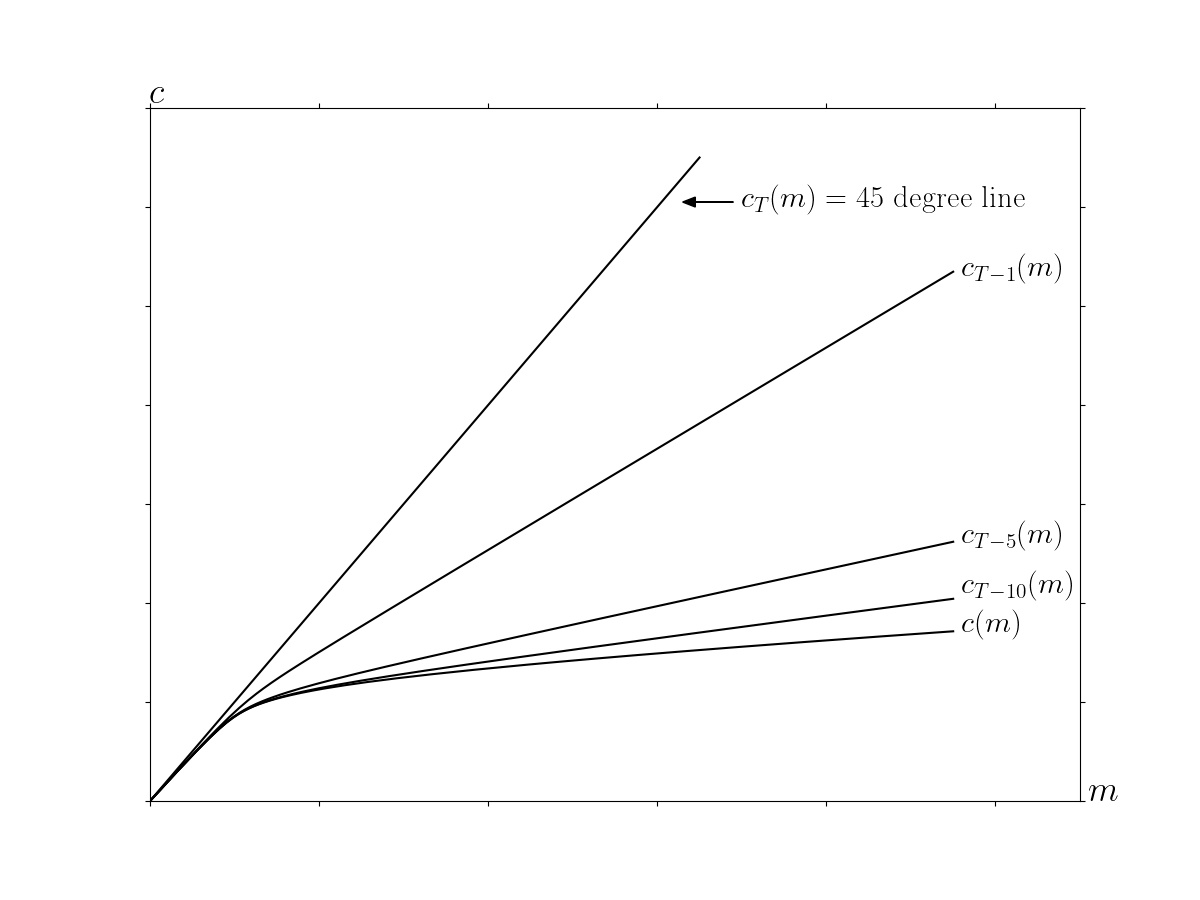
\includegraphics[width=5.25in]{\FigDir/cFuncsConverge}}
\caption{Convergence of the Consumption Rules}
\label{fig:cFuncsConverge}
\end{figure}

\begin{figure}[ht]
  \centerline{
    
\includegraphics[width=6.0in]{\FigDir/Inequalities}
  }
  \caption{Relation of All Inequality Conditions} \label{fig:Inequalities}
\centerline{See Table~\ref{table:Calibration} for Numerical Values of Nodes Under Baseline Parameters}
\end{figure}

\hypertarget{FVACnotGIC}{}
\begin{figure}[tbp]
\centerline{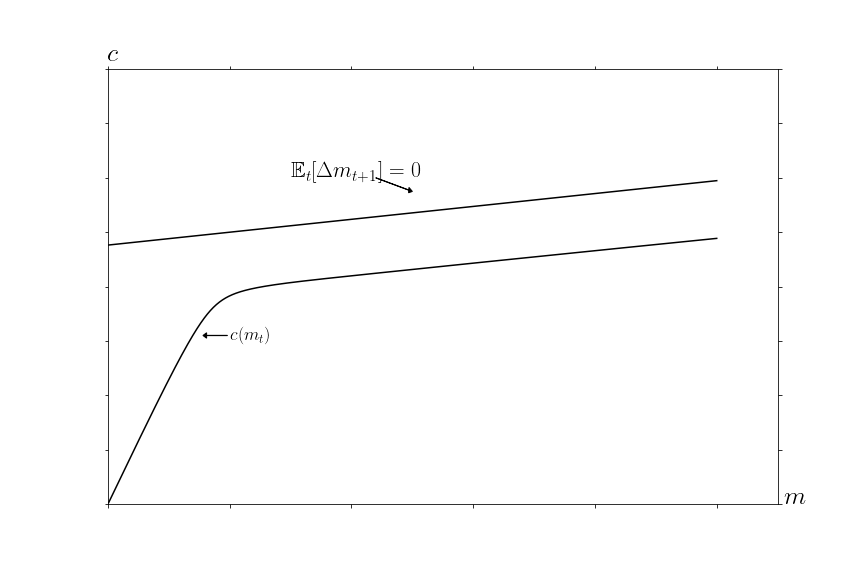
\includegraphics[width=6in]{\FigDir/FVACnotGIC}}
\caption{Example Solution under \{{FVAC},\cncl{GIC-Mod}\}}
\label{fig:FVACnotGIC}
\end{figure}

% Could not get fonts to work right for svg version of this figure for web; so use png
\ifthenelse{\boolean{Web}}{
\begin{figure}[tbp]
\centerline{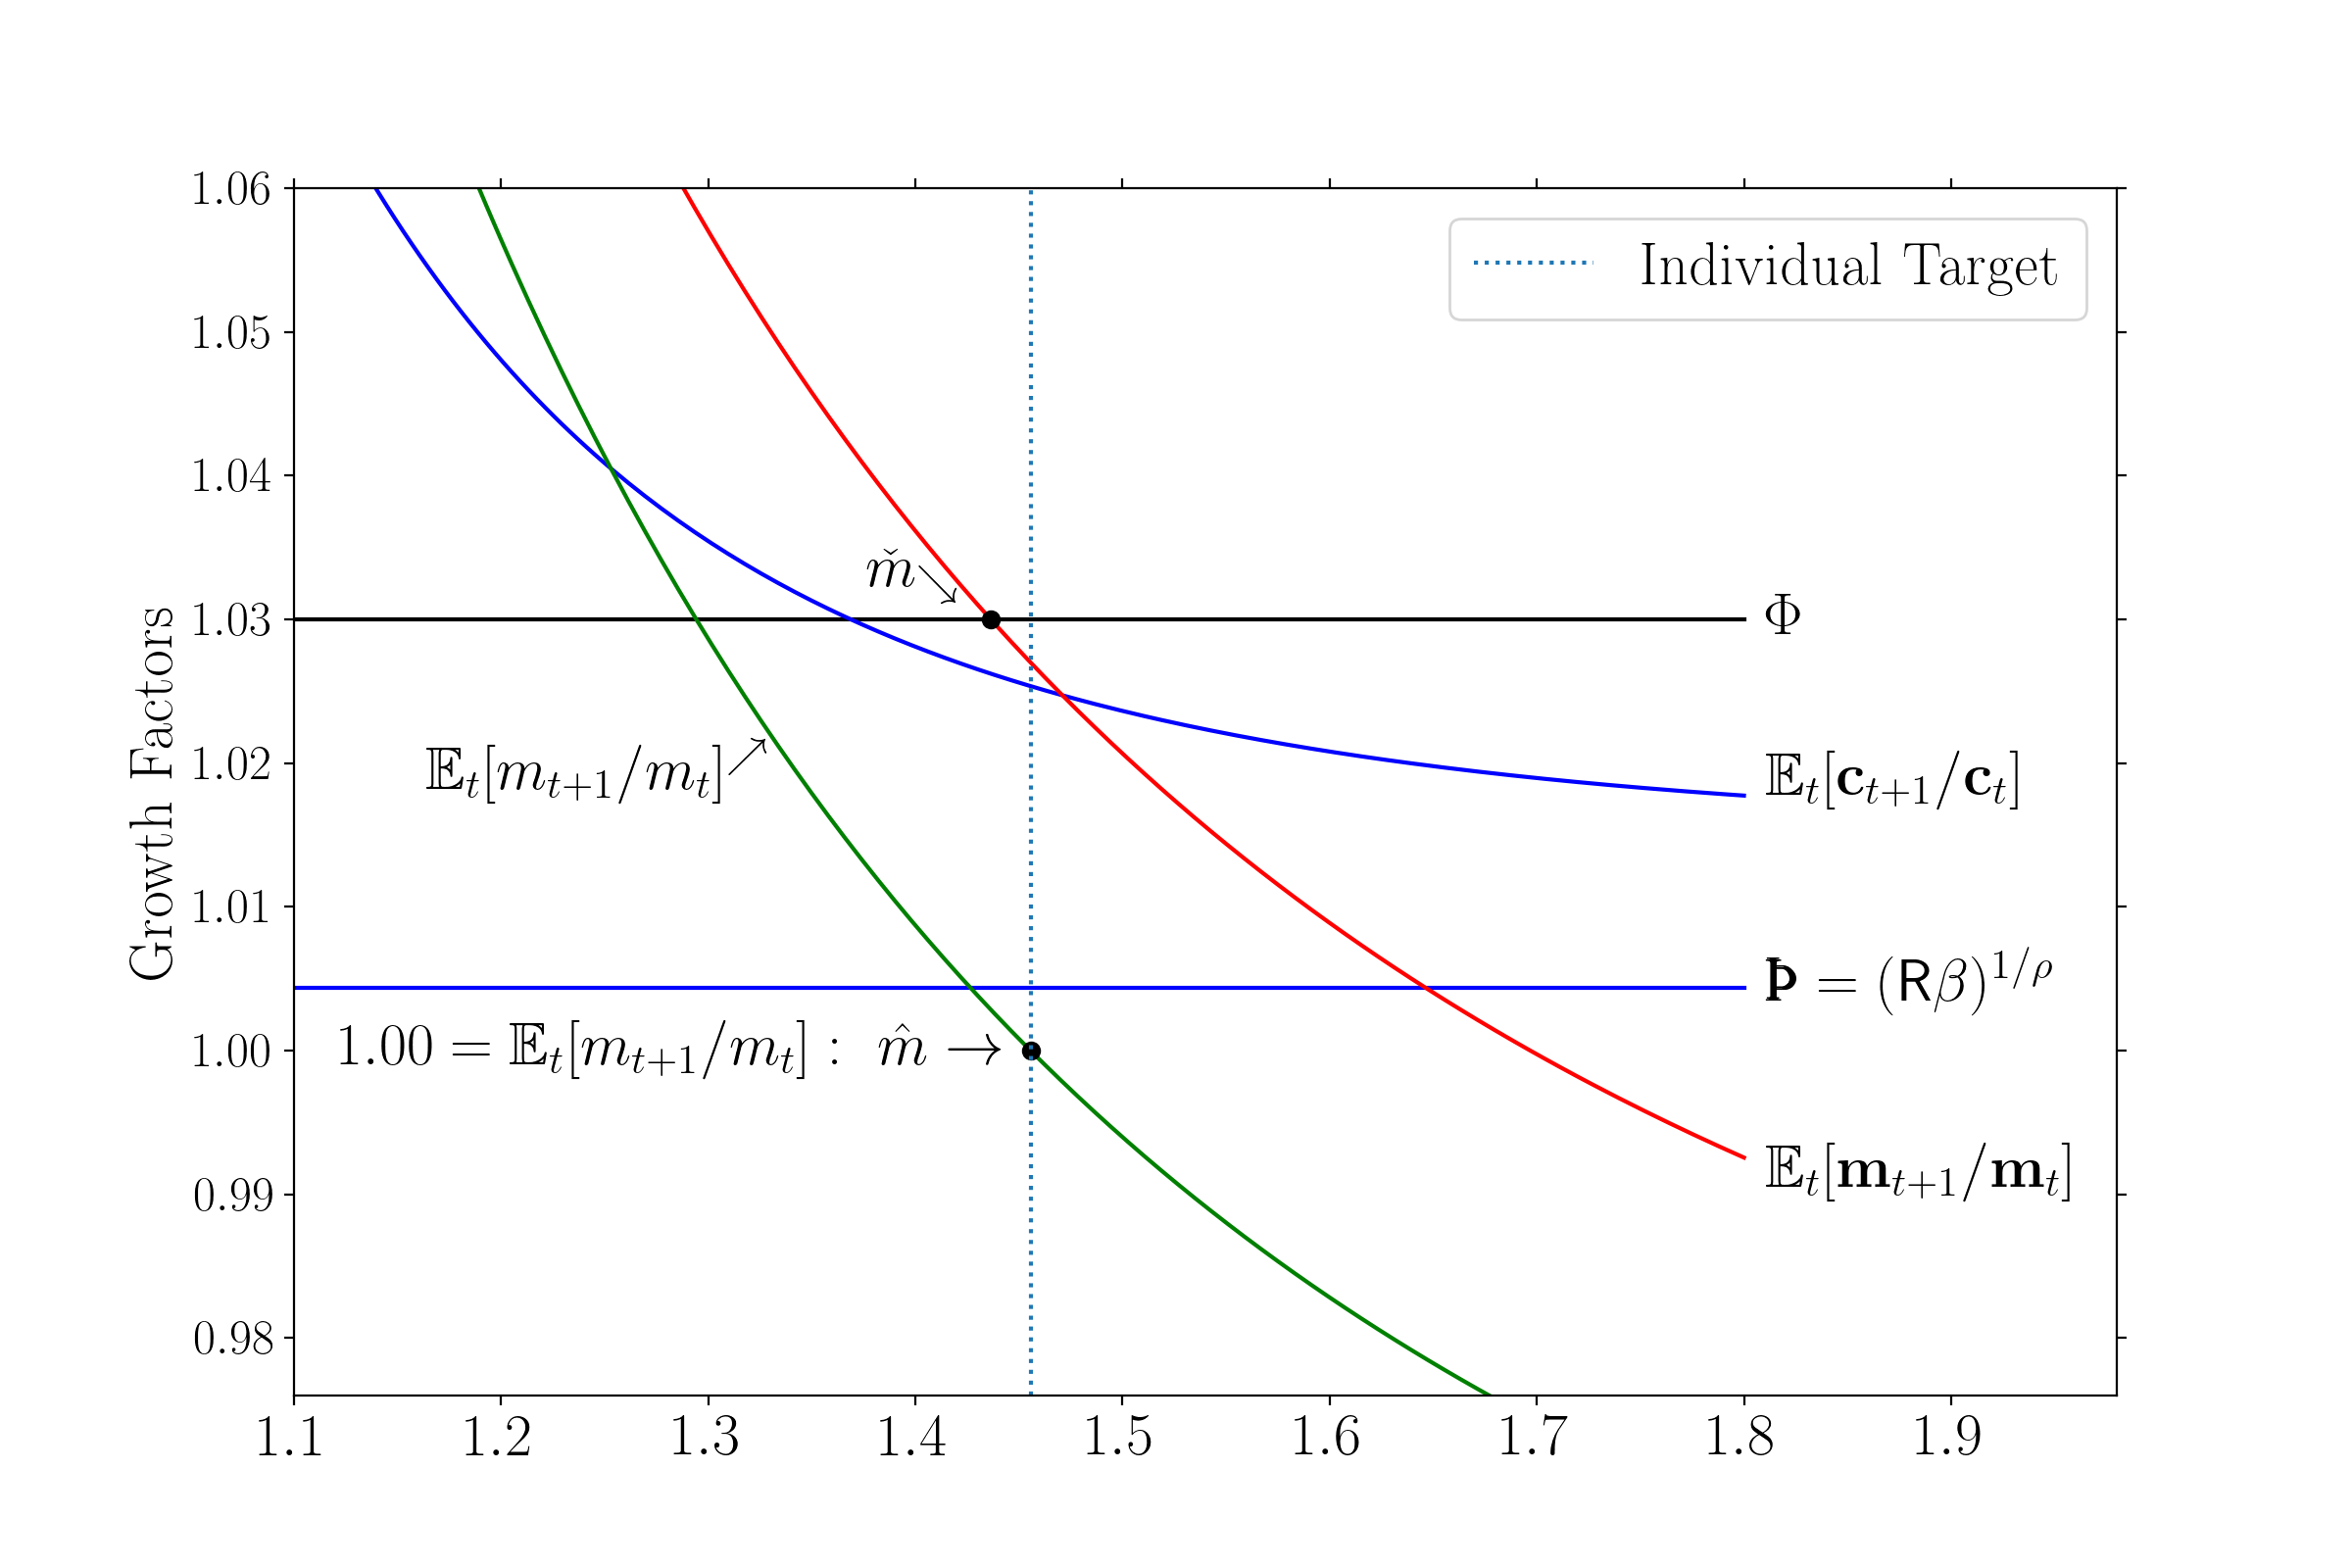
\includegraphics[width=8in]{\FigDir/cNrmTargetFig.png}}
\caption{`Stable' $\mNrm$ Values and Expected Growth Rates}
\label{fig:cNrmTargetFig}
\end{figure}
}{
\begin{figure}[tbp]
\centerline{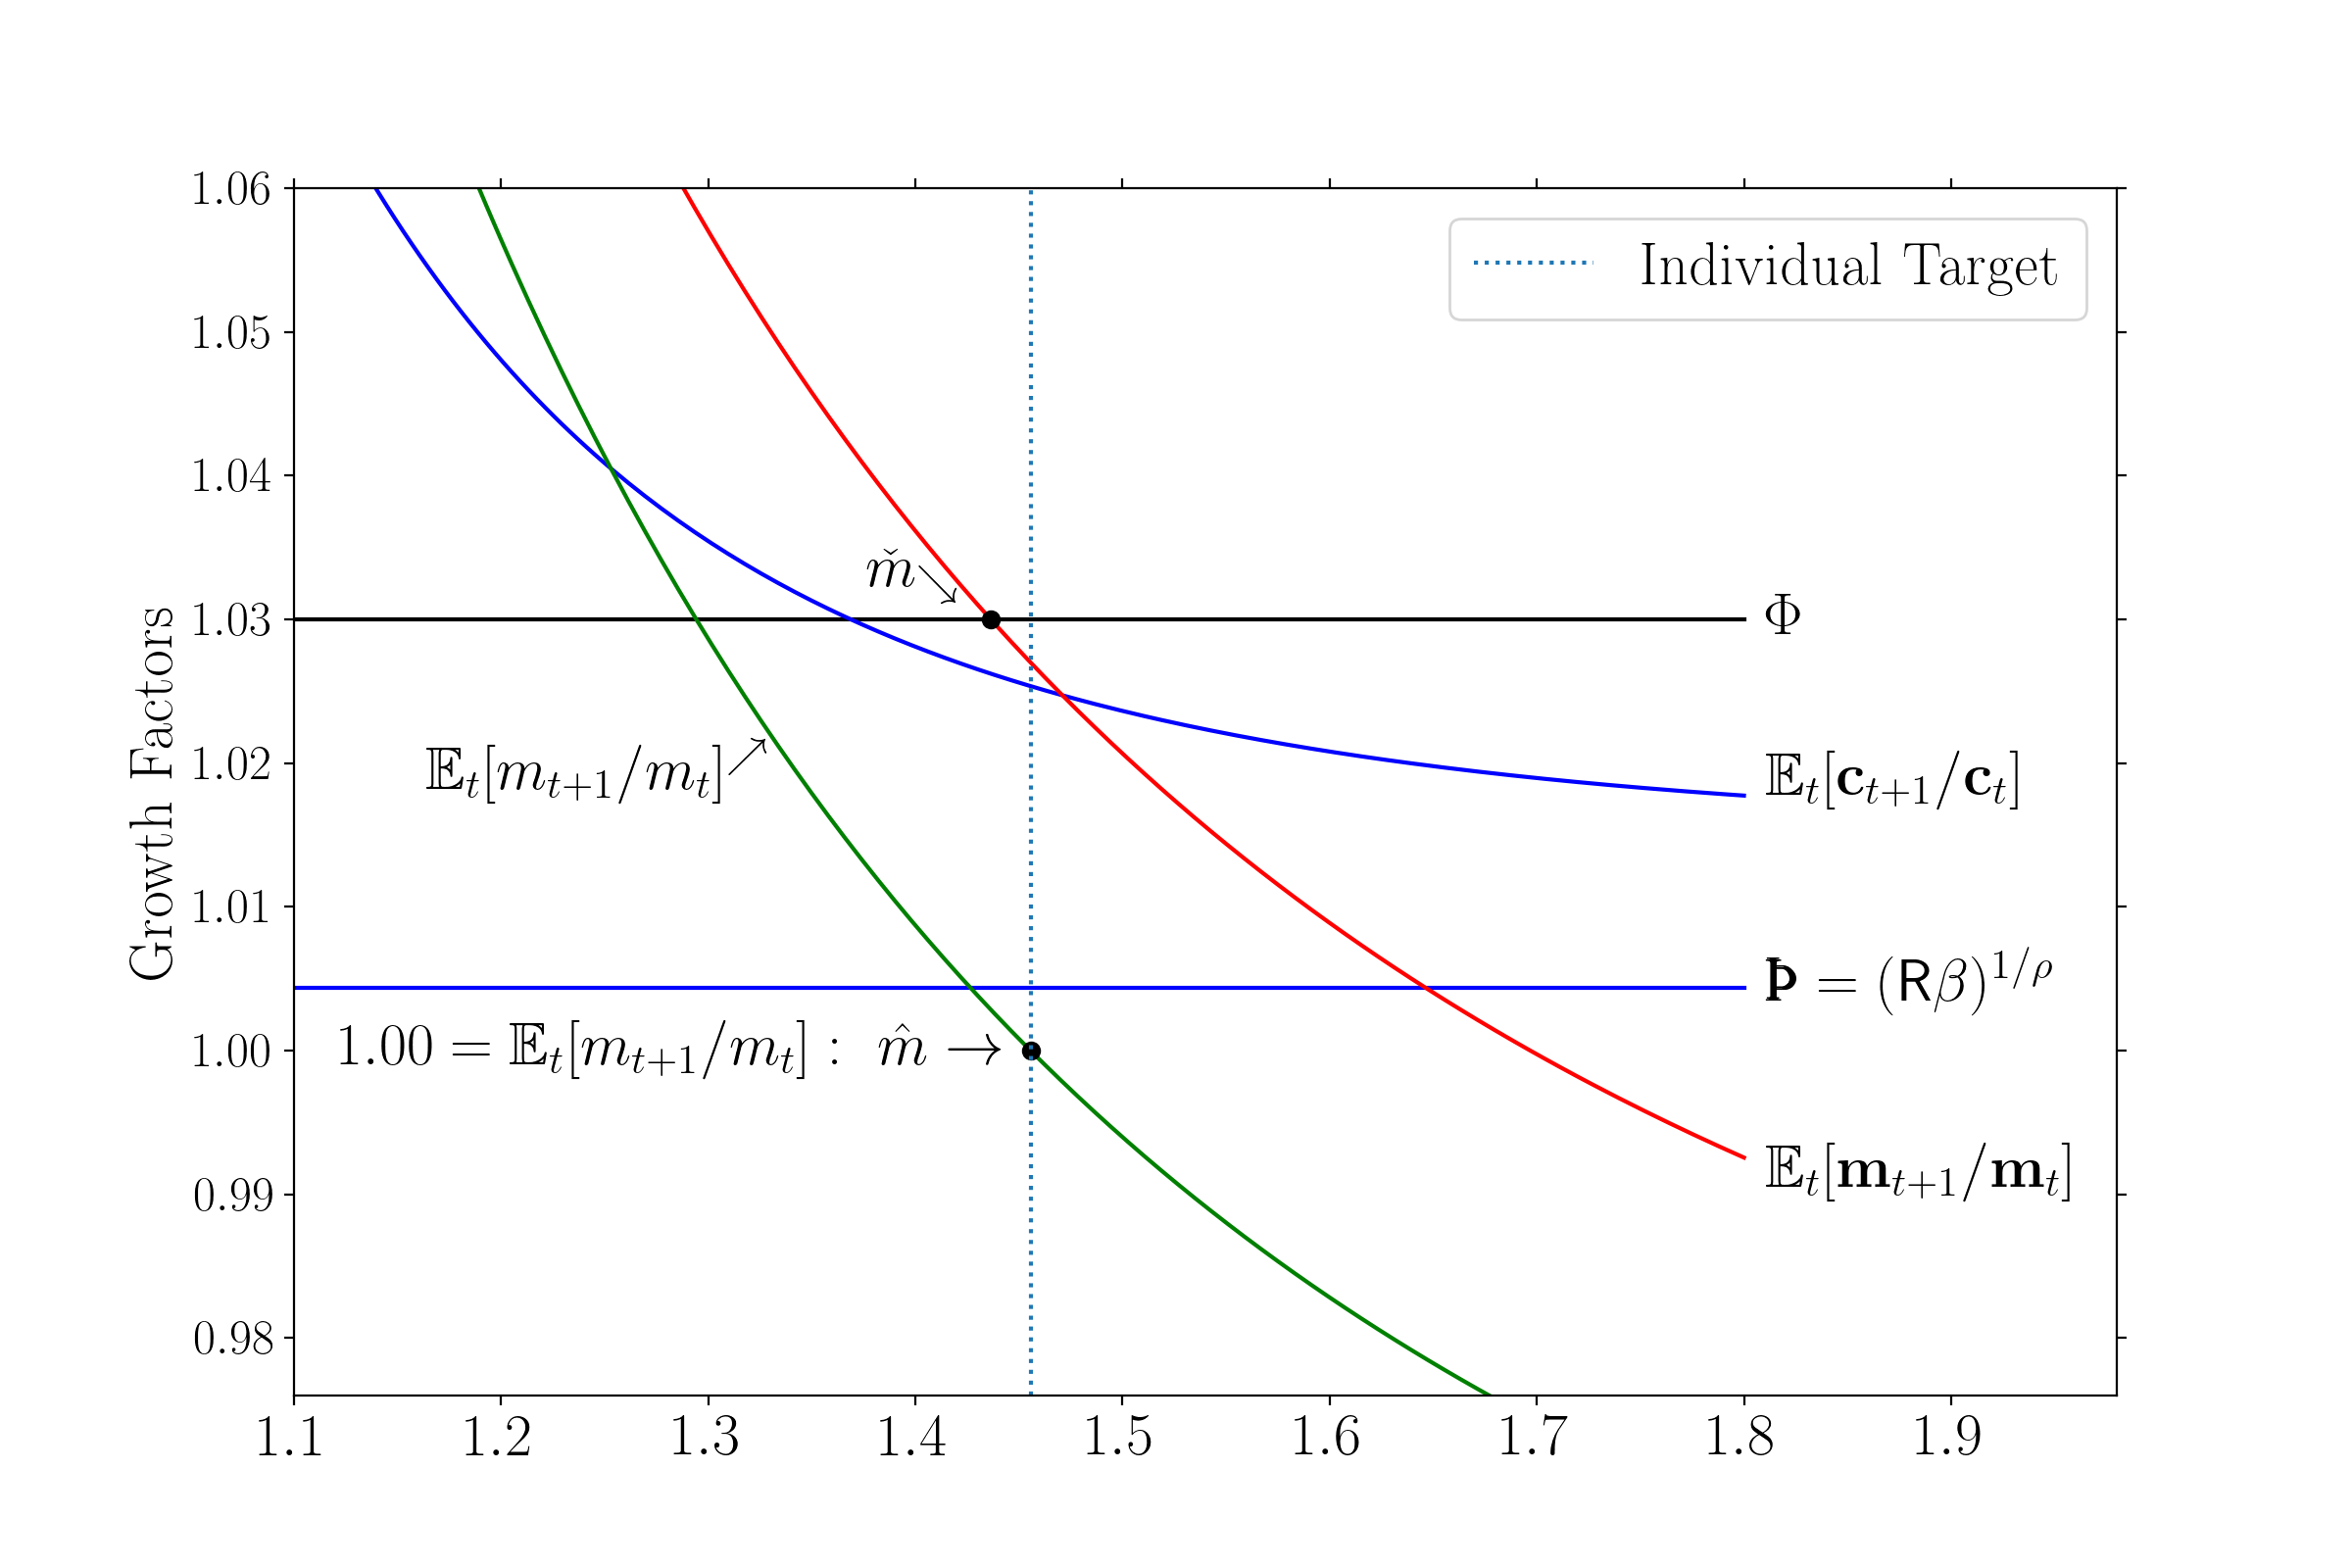
\includegraphics[width=6in]{\FigDir/cNrmTargetFig}}
\caption{`Stable' (Target; Balanced Growth) $\mNrm$ Values}
\label{fig:cNrmTargetFig}
\end{figure}
}

\hypertarget{MPCLimits}{}
\begin{figure}
\centerline{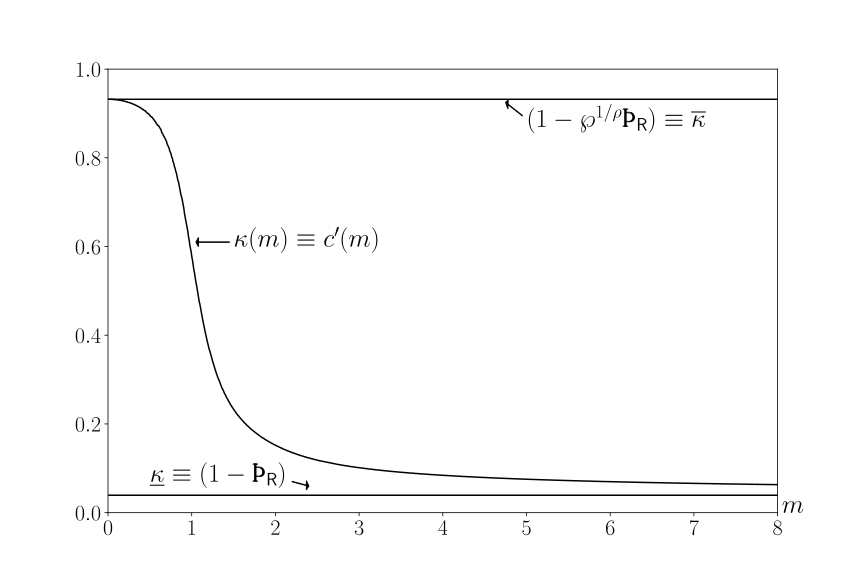
\includegraphics[width=6in]{\FigDir/MPCLimits}}
\caption{Limiting MPC's}
\label{fig:mpclimits}
\end{figure}

\hypertarget{cFuncBounds}{}
\begin{figure}
\centering
\subfigure[\large Bounds]{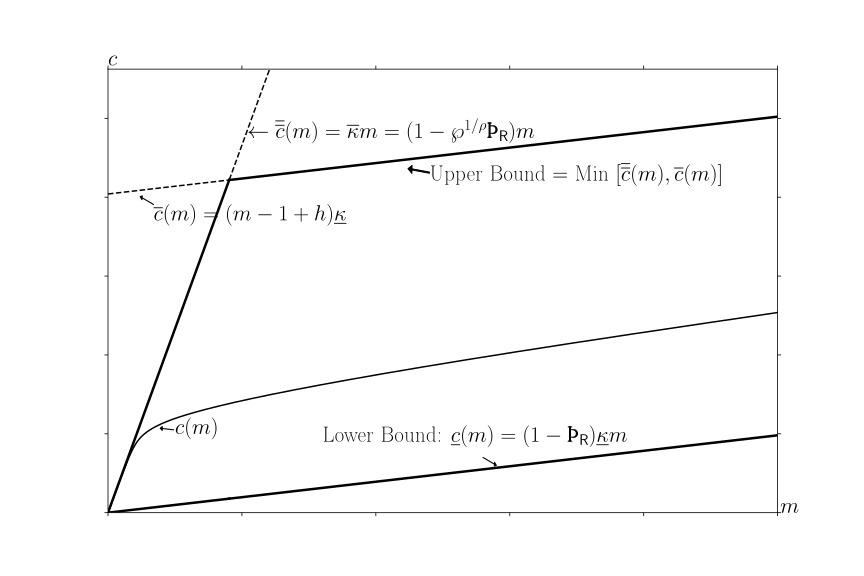
\includegraphics[width=6in]{\FigDir/cFuncBounds}}
\subfigure[\large Target $\mNrm$]{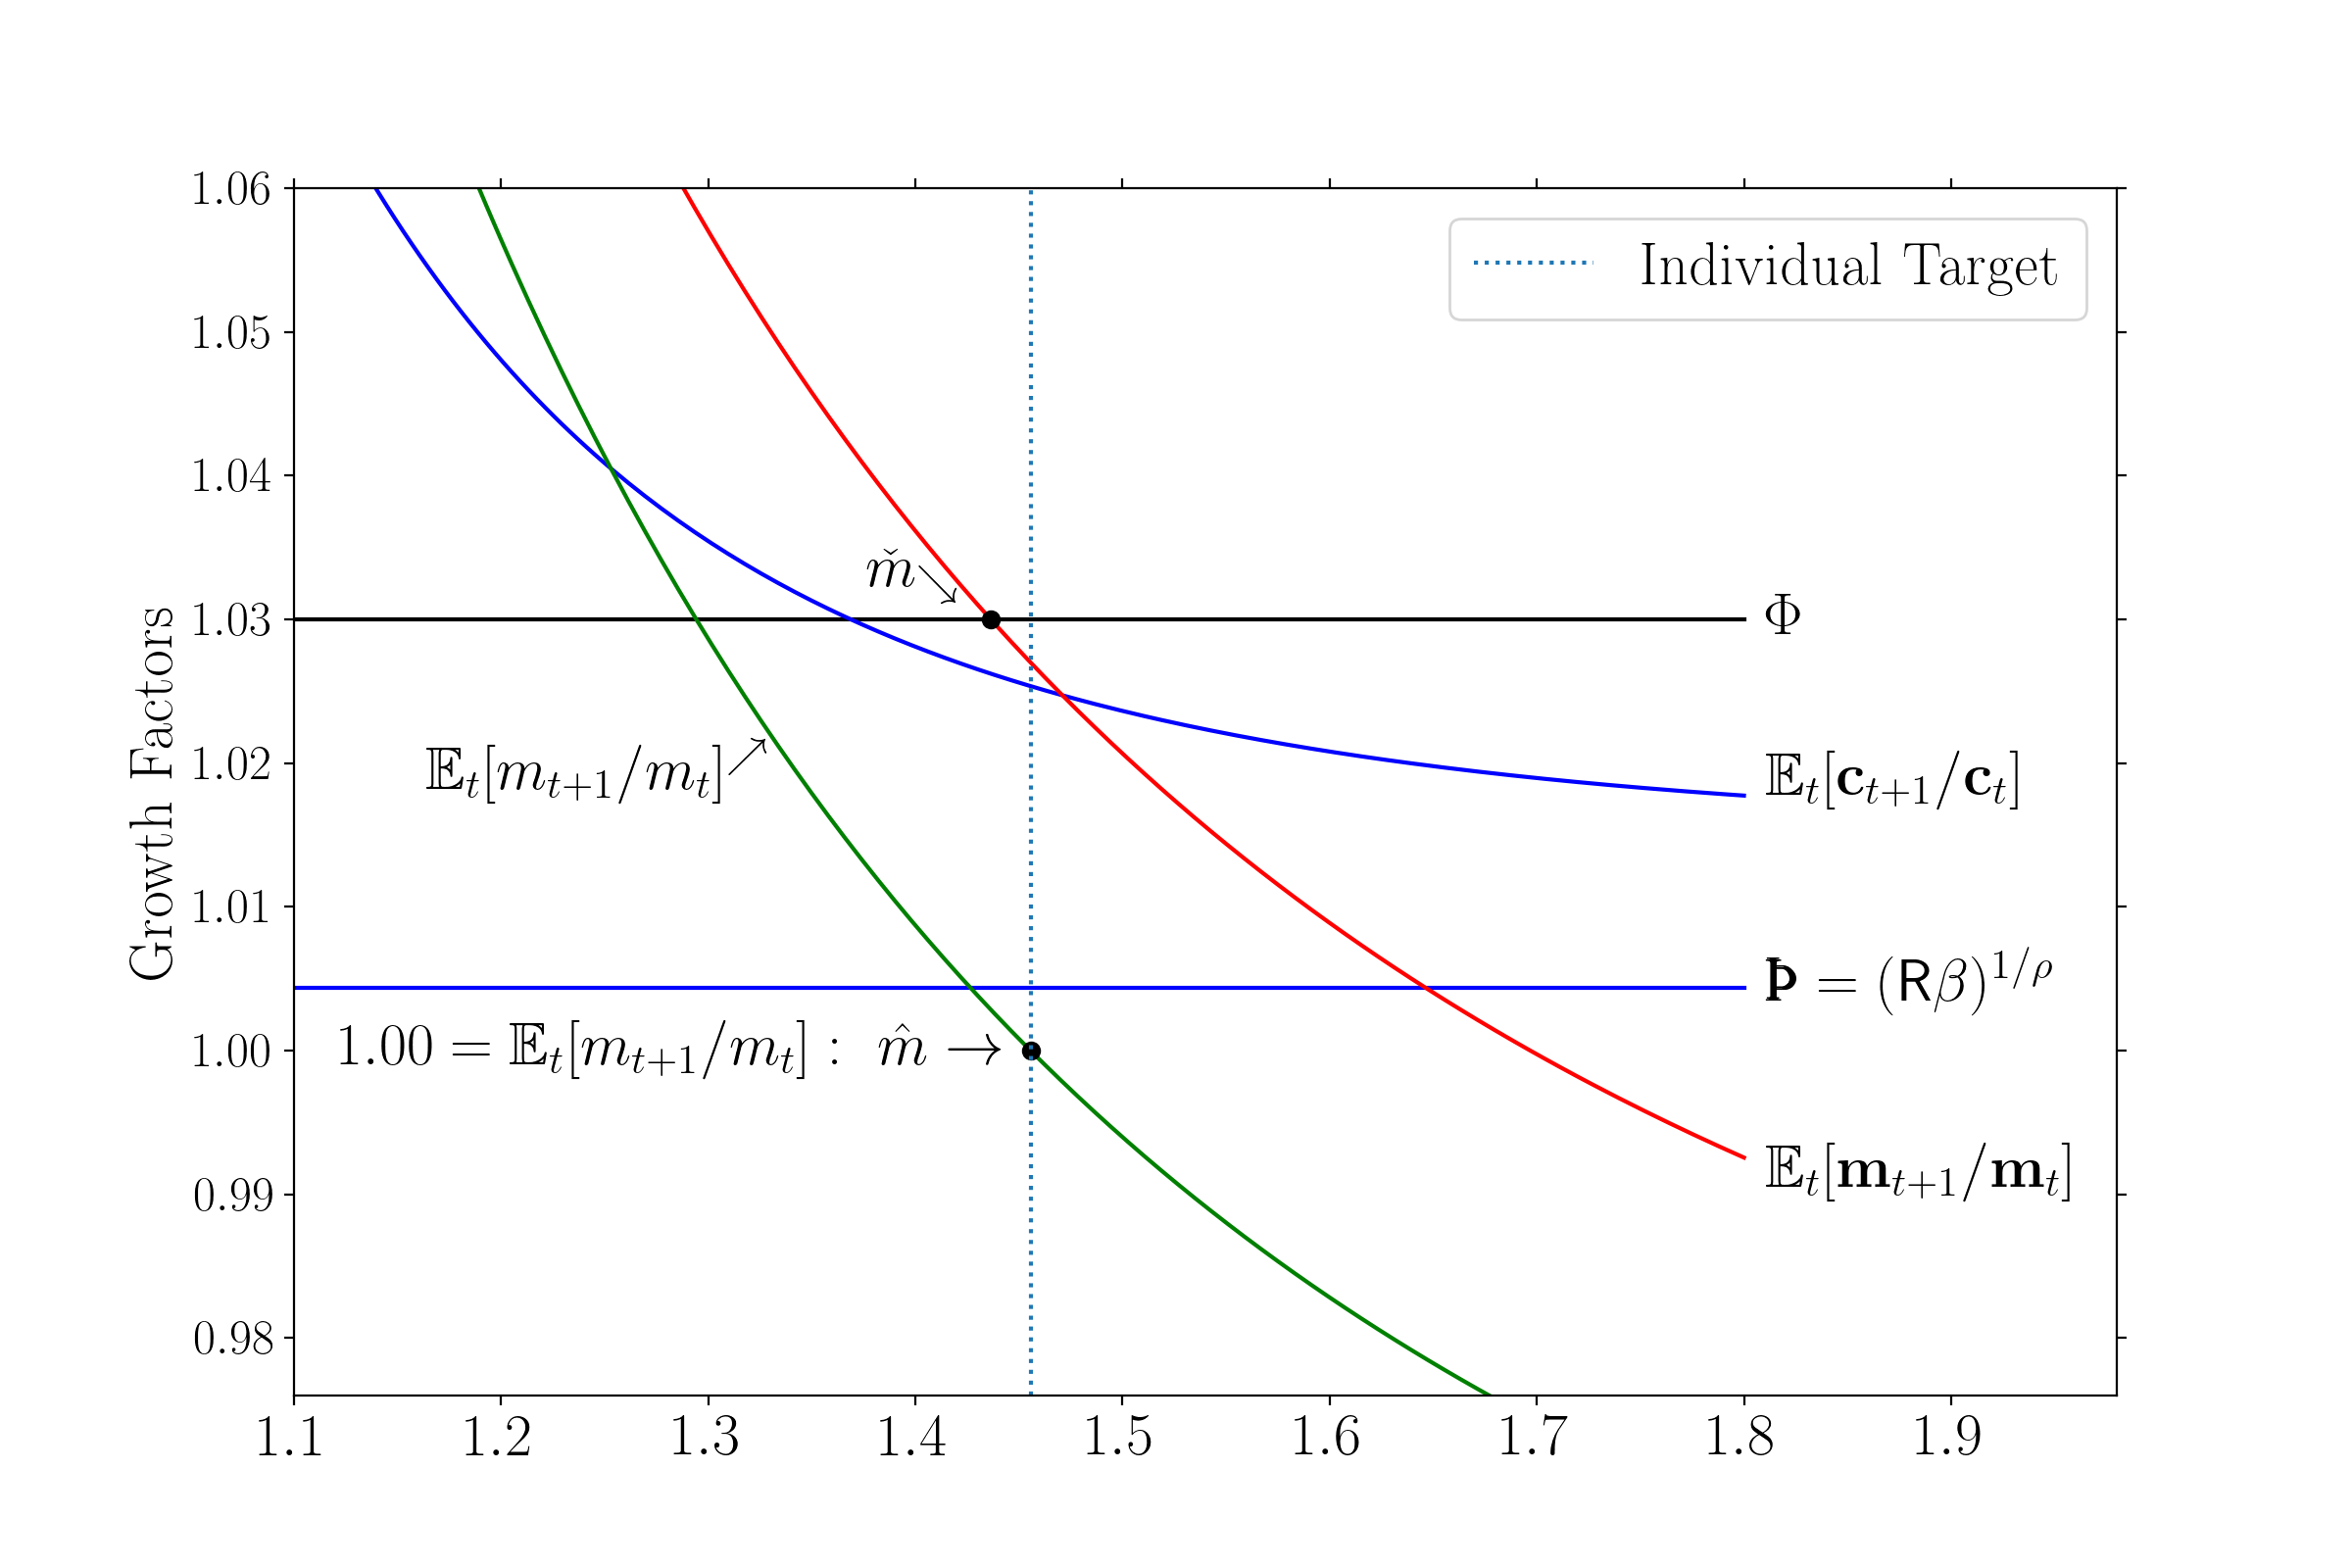
\includegraphics[width=6in]{\FigDir/cNrmTargetFig}}
\caption{The Consumption Function}
\label{fig:cFuncBounds}
\end{figure}

\hypertarget{PFGICHoldsFHWCFailsRICFails}{}
\begin{figure}
\centerline{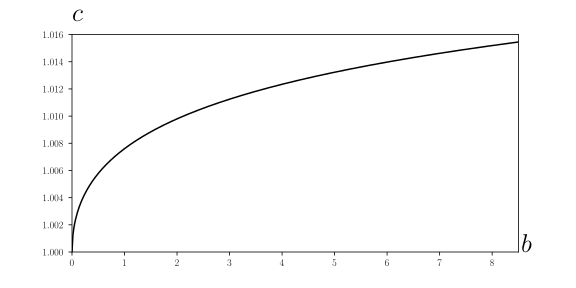
\includegraphics[width=6in]{\FigDir/PFGICHoldsFHWCFailsRICFails}}
\caption{Appendix: Nondegenerate $\cFunc$ Function with \cncl{FHWC} and \cncl{RIC}}
\label{fig:PFGICHoldsFHWCFailsRICFails}
\end{figure}



\end{document}
% Local Variables:
% eval: (setq TeX-command-list  (assq-delete-all (car (assoc "BibTeX" TeX-command-list)) TeX-command-list))
% eval: (setq TeX-command-list  (assq-delete-all (car (assoc "BibTeX" TeX-command-list)) TeX-command-list))
% eval: (setq TeX-command-list  (assq-delete-all (car (assoc "BibTeX" TeX-command-list)) TeX-command-list))
% eval: (setq TeX-command-list  (assq-delete-all (car (assoc "BibTeX" TeX-command-list)) TeX-command-list))
% eval: (setq TeX-command-list  (assq-delete-all (car (assoc "Biber"  TeX-command-list)) TeX-command-list))
% eval: (add-to-list 'TeX-command-list '("BibTeX" "bibtex ../LaTeX/%s" TeX-run-BibTeX nil t                                                                              :help "Run BibTeX") t)
% eval: (add-to-list 'TeX-command-list '("BibTeX" "bibtex ../LaTeX/%s" TeX-run-BibTeX nil (plain-tex-mode latex-mode doctex-mode ams-tex-mode texinfo-mode context-mode) :help "Run BibTeX") t)
% tex-bibtex-command: "bibtex ../LaTeX/*"
% TeX-PDF-mode: t
% TeX-file-line-error: t
% TeX-debug-warnings: t
% LaTeX-command-style: (("" "%(PDF)%(latex) %(file-line-error) %(extraopts) -output-directory=../LaTeX %S%(PDFout)"))
% TeX-source-correlate-mode: t
% TeX-parse-self: t
% eval: (cond ((string-equal system-type "darwin") (progn (setq TeX-view-program-list '(("Skim" "/Applications/Skim.app/Contents/SharedSupport/displayline -b %n ../LaTeX/%o %b"))))))
% eval: (cond ((string-equal system-type "gnu/linux") (progn (setq TeX-view-program-list '(("Evince" "evince --page-index=%(outpage) ../LaTeX/%o"))))))
% eval: (cond ((string-equal system-type "gnu/linux") (progn (setq TeX-view-program-selection '((output-pdf "Evince"))))))
% TeX-parse-all-errors: t
% End:
